\actTitle{1.4 - Lines}

\videoLink{Section 1.4}{https://www.youtube.com/playlist?list=PLYHZK3b8UFw0jGzT4r6nABTLh3CI6eVst}

\noindent \textbf{Topics:}  Equations of lines, parallel and perpendicular lines, linear models, average rate of change\\

\noindent \textbf{Student Learning Outcomes:}
\begin{enumerate}
\item Students will be able to graph linear equations.
\item Students will be able to determine the slope of a line and apply the slope-intercept form of a line.
\item Students will be able to compute the average rate of change of a function.
\end{enumerate}

\hrule 

\bigskip

\subsection{Slope of a Line} ~

\noindent 
\begin{tabular}{| l |} \hline
The \underline{slope of a line} is $m = \dfrac{y_2-y_1}{x_2-x_1}$.  \\ \hline
 \end{tabular} 
 



\begin{enumerate}
\item Sketch the line through the pair of points $P(4,2)$ and $Q(-3,5
)$, and find the slope of the line. 

      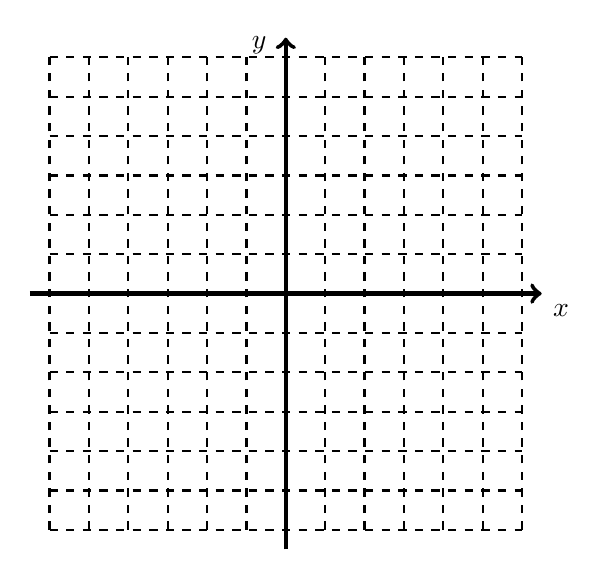
\begin{tikzpicture}[y=0.5cm, x=0.5cm,font=\sffamily]
        \begin{scope} %[shift={(0,8)}]
          %% ticks
          \draw[xstep = 1, ystep=1.0,black,dashed,thick] % very thin,opacity=0.85,
                 (-6.0,-6.0) grid ( 6.0, 6.0);
             %% axis
           \draw[ultra thick,->] (-6.5,0) -- coordinate (x axis mid) (6.5,0)
                node[anchor = north west] {$x$}; 
           \draw[ultra thick,->] (0,-6.5) -- coordinate (y axis mid) (0,6.5) 
                node[anchor = east,shift={(-0.2,-0.2)}]  {$y$};

           %\foreach \y in {-1,1,...,4} {
           %   \draw (1pt, \y) -- (-1pt, \y) node[yshift=-6,xshift=1,anchor=west] {$\y$};
           % }
           %\foreach \x in {-3,-2,-1,1,2,3} {
           %   \draw (\x,1pt) -- (\x,-1pt) node[yshift=-5,xshift=-1,anchor=east] {$\x$};
           % }

          \end{scope}
        \end{tikzpicture}

\hspace{-.3in} \begin{tabular}{| l |}\hline
 \noindent The \underline{point-slope equation} for the line through the point $(x_1,y_1)$ with slope $m$ is \\

 $y-y_1 = m(x-x_1)$. \\ \hline
\end{tabular} 

\vspace{-.1in}
\item Determine a \emph{point-slope} equation for the line through $P(4,2)$ and $Q(-3,5)$.(See above.)\\[1in]






\hspace{-.3in} \begin{tabular}{| l |}\hline The \underline{slope-intercept equation} for the line with slope $m$ and $y$-intercept $b$ is \\

 $y = mx +b$. \\ \hline
\end{tabular} 



\vspace{-.1in}
\item Determine the \emph{slope-intercept} equation for the line through $(3, -2)$ which has slope $-4$. \\[1in]



\noindent \textbf{Horizontal lines} have 0 slope and \textbf{vertical lines} have undefined slopes.\\[1in]


\subsection{Parallel and Perpendicular Lines} ~

\hspace{-.3in} \begin{tabular}{| l |  }
\hline Parallel lines have the \emph{same slope.} \\ \hline
\end{tabular} %\\[.5in]

\vspace{-.1in}
\item Determine a point-slope equation for the line through $(-1,2)$ which is parallel to the line $2x + 3y - 5 = 0$ and graph the equation.

      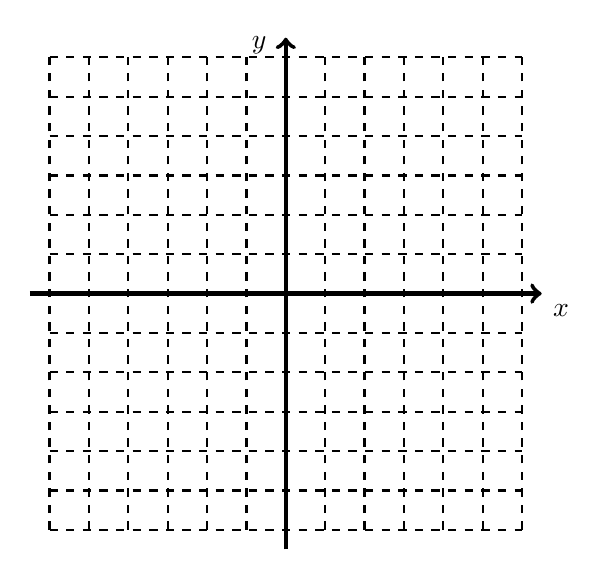
\begin{tikzpicture}[y=0.5cm, x=0.5cm,font=\sffamily]
        \begin{scope} %[shift={(0,8)}]
          %% ticks
          \draw[xstep = 1, ystep=1.0,black,dashed,thick] % very thin,opacity=0.85,
                 (-6.0,-6.0) grid ( 6.0, 6.0);
             %% axis
           \draw[ultra thick,->] (-6.5,0) -- coordinate (x axis mid) (6.5,0)
                node[anchor = north west] {$x$}; 
           \draw[ultra thick,->] (0,-6.5) -- coordinate (y axis mid) (0,6.5) 
                node[anchor = east,shift={(-0.2,-0.2)}]  {$y$};

           %\foreach \y in {-1,1,...,4} {
           %   \draw (1pt, \y) -- (-1pt, \y) node[yshift=-6,xshift=1,anchor=west] {$\y$};
           % }
           %\foreach \x in {-3,-2,-1,1,2,3} {
           %   \draw (\x,1pt) -- (\x,-1pt) node[yshift=-5,xshift=-1,anchor=east] {$\x$};
           % }

          \end{scope}
        \end{tikzpicture}



\clearpage

\hspace{-.3in}\begin{tabular}{| l |  }
\hline Perpendicular lines have slopes that are ``negative reciprocals" of each other. If $m_1$ is the \\ slope of one of the lines, then the slope of the other line must be $-1/m_1$. \\ \hline
\end{tabular} 

\item Determine an equation of the line through the point $(-3, 1)$ which is perpendicular to the line $2x+4y+7=0$ and graph the equation.

      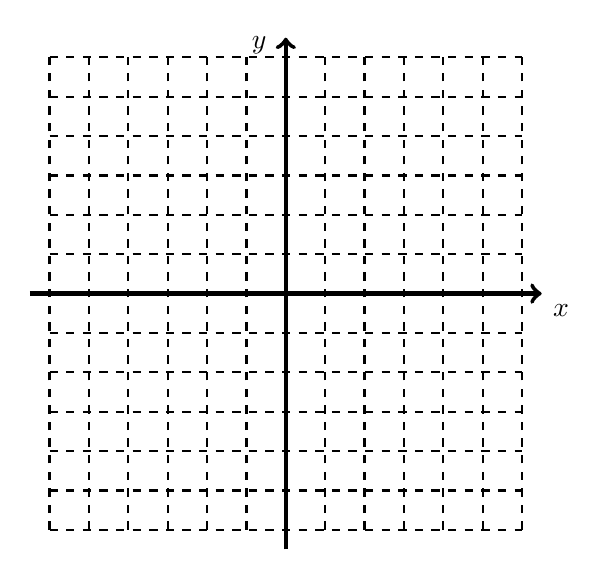
\begin{tikzpicture}[y=0.5cm, x=0.5cm,font=\sffamily]
        \begin{scope} %[shift={(0,8)}]
          %% ticks
          \draw[xstep = 1, ystep=1.0,black,dashed,thick] % very thin,opacity=0.85,
                 (-6.0,-6.0) grid ( 6.0, 6.0);
             %% axis
           \draw[ultra thick,->] (-6.5,0) -- coordinate (x axis mid) (6.5,0)
                node[anchor = north west] {$x$}; 
           \draw[ultra thick,->] (0,-6.5) -- coordinate (y axis mid) (0,6.5) 
                node[anchor = east,shift={(-0.2,-0.2)}]  {$y$};

           %\foreach \y in {-1,1,...,4} {
           %   \draw (1pt, \y) -- (-1pt, \y) node[yshift=-6,xshift=1,anchor=west] {$\y$};
           % }
           %\foreach \x in {-3,-2,-1,1,2,3} {
           %   \draw (\x,1pt) -- (\x,-1pt) node[yshift=-5,xshift=-1,anchor=east] {$\x$};
           % }

          \end{scope}
        \end{tikzpicture}


\subsection{Average Rate of Change}
\textbf{Average Rate of Change}\\
Given any function $y=f(x)$, we calculate the average rate of change of $y$ with respect to $x$ over the interval  $[x_1,x_2]$ by dividing the change in value of $y$, $\Delta y=f(x_2)-f(x_1)$, by the length  $\Delta x=x_2-x_1$ of the interval over which the change occurs.\\


 The \textbf{\emph{average rate of change}} of $y=f(x)$ with respect to $x$ over the interval $[x_1,x_2]$ is
 $$\frac{\Delta y}{\Delta x}=\frac{y_2-y_1}{x_2-x_1}=\frac{f(x_2)-f(x_1)}{x_2-x_1}$$\\ 
 
\noindent \textbf{Note:  }An average rate of change needs two points (or endpoints on an interval). 






\item Given the function defined $f(x)=x^2-1$, determine the average rate of change from $x_1=-2$ to $x_2=0.$\\[2in]


\end{enumerate}

\noindent \textbf{Student Learning Outcomes Check}

\begin{enumerate}
\item Can you graph a linear equation?
\item Can you determine the slope of a line and apply the slope-intercept form of a line?
\item Can you compute the average rate of change of a function?
\end{enumerate}

\noindent \textbf{If any of your answers were no, please ask about these topics in class.}

